%%%%%%%%%%%%%%%%%%%%%%%%%%%%%%%%%%%%%%%%%
% Beamer Presentation
% LaTeX Template
% Version 1.0 (10/11/12)
%
% This template has been downloaded from:
% http://www.LaTeXTemplates.com
%
% License:
% CC BY-NC-SA 3.0 (http://creativecommons.org/licenses/by-nc-sa/3.0/)
%
%%%%%%%%%%%%%%%%%%%%%%%%%%%%%%%%%%%%%%%%%

%----------------------------------------------------------------------------------------
%	PACKAGES AND THEMES
%----------------------------------------------------------------------------------------

\documentclass{beamer}

\mode<presentation> {

% The Beamer class comes with a number of default slide themes
\usetheme{Madrid}

\setbeamertemplate{navigation symbols}{} % To remove the navigation symbols from the bottom of all slides uncomment this line
}

\usepackage{graphicx} % Allows including images
\usepackage{booktabs} % Allows the use of \toprule, \midrule and \bottomrule in tables
\usepackage{amsmath}
\usepackage{braket}
\usepackage{hyperref}

\hypersetup{
    colorlinks=true
}

%shortcuts
\renewcommand{\C}{\mathbb{C}}

%----------------------------------------------------------------------------------------
%	TITLE PAGE
%----------------------------------------------------------------------------------------

\title[Intro to Quantum]{Quantum Computing: An Intro} % The short title appears at the bottom of every slide, the full title is only on the title page

\author{Heman Gandhi} % Your name
\institute[Rutgers] % Your institution as it will appear on the bottom of every slide, may be shorthand to save space
{
 Rutgers -- HackRU RnD\\ % Your institution for the title page
\medskip
\textit{hemang@ndhi.ninja} % Your email address
}
\date{\today} % Date, can be changed to a custom date

\begin{document}

\begin{frame}
\titlepage % Print the title page as the first slide
\end{frame}

\begin{frame}
\frametitle{Overview} % Table of contents slide, comment this block out to remove it
\tableofcontents % Throughout your presentation, if you choose to use \section{} and \subsection{} commands, these will automatically be printed on this slide as an overview of your presentation
\end{frame}

%----------------------------------------------------------------------------------------
%	PRESENTATION SLIDES
%----------------------------------------------------------------------------------------

%------------------------------------------------
\section{Intro: what is this presentation} % Sections can be created in order to organize your presentation into discrete blocks, all sections and subsections are automatically printed in the table of contents as an overview of the talk
%------------------------------------------------

\begin{frame}
\frametitle{UwU, What This?}
This is an intro to quantum computing.
So what I'll be doing is going over brief,
sometimes not very technical answers to the following (in chronological order):
\begin{itemize}
    \item What is quantum computing?
    \item What are some questions people are asking about it?
    \item Some Math
    \item Where can I go to mess with quantum computing?
\end{itemize}
\end{frame}

\begin{frame}
\frametitle{What is Quantum Computing?}

(See \cite{5-levels} for more.)

\begin{block}{To a Child:}
Computers represent computers as coins with ``heads'' and ``tails''. A quantum computer also lets you rotate the coin.
\end{block}

\begin{block}{To a Teen:}
Superposition is like trying to tell if a coin if heads or tails while it's being tossed.

Entanglement is when two coins are forced to have the same state.
\end{block}
\end{frame}

\section{QC Applications and Questions}

\begin{frame}
\frametitle{How to use this?}
This is a subset:
\begin{itemize}
    \item Fast factoring (Shor's Algorithm)
    \item Computational (micro)-biology
    \item Quantum Machine Learning
    \item Quantum Cryptography
\end{itemize}
\end{frame}

\begin{frame}
\frametitle{How to Measure the Benefit?}
There is a field called Quantum complexity theory. We know that quantum computers are at most exponentially faster
from this.

We also get that we can solve circuit satisfiability in a square-root of the time (with an error bound).

Searches are also theorized to be in a square-root of the time. \cite{q-complexity}

Only recently can we verify whether a quantum computer even used quantum magic to compute. \cite{q-verification}
\end{frame}

\begin{frame}
\frametitle{Open Questions}
Some of the open questions are:
\begin{itemize}
    \item How to implement\dots anything?
    \item What should programming languages look like?
    \item How to scale quantum computers to match the requirements?
\end{itemize}

There are many, many more!
\end{frame}

\section{QC Basics}

\begin{frame}
\frametitle{More rigorously...}

This is why I used \LaTeX.
Much of what follows about how Q-bits work is thanks to \cite{long-video}.

\begin{definition}
    We write bits as vectors. So $\begin{pmatrix}1 \\ 0\end{pmatrix}$ is the $0$ bit,
    written in ``Dirac notation'' as
    $\ket{0}$.
\end{definition}

Any guesses about representing a 1-bit?
\end{frame}

\begin{frame}
\frametitle{Classical Systems}
\begin{table}
\begin{tabular}{l l l}
\toprule
\textbf{Bit} & \textbf{As a Vector} & \textbf{Dirac Notation}\\
\midrule
1 & $\begin{pmatrix}0 \\ 1\end{pmatrix}$ & $\ket{1}$ \\
0 & $\begin{pmatrix}1 \\ 0\end{pmatrix}$ & $\ket{0}$ \\
\bottomrule
\end{tabular}
\caption{The Classical Bit States}
\end{table}

Mnemonic: the Dirac notation gives you the index of the 1 in the vector.
\end{frame}

\begin{frame}
\frametitle{Matrix Multiplication as Bit Operators}
Bit operations can be thought of
as certain matrices.

\begin{table}
\begin{tabular}{l l}
\toprule
\textbf{Bit Operation} & \textbf{Matrix}\\
\midrule
Identity & $\begin{pmatrix}1 & 0 \\ 0 & 1\end{pmatrix}$ \\
Not & $\begin{pmatrix}0 & 1 \\ 1 & 0\end{pmatrix}$\\
Set to 0 & $\begin{pmatrix}1 & 1 \\ 0 & 0\end{pmatrix}$\\
Set to 1 & $\begin{pmatrix}0 & 0 \\ 1 & 1\end{pmatrix}$\\
\bottomrule
\end{tabular}
\caption{The Classical Unary Bitwise Operators}
\end{table}

What does invertibility mean here?

\end{frame}


\begin{frame}
\frametitle{$\bigotimes$: Tensors}

\begin{columns}[c] % The "c" option specifies centered vertical alignment while the "t" option is used for top vertical alignment

\column{.5\textwidth} % Left column and width

\begin{definition}[Tensor Product of vectors]
    $\begin{pmatrix}x_0 \\ \vdots \\ x_n\end{pmatrix} \otimes \begin{pmatrix}y_0 \\ \vdots \\ y_m\end{pmatrix} = \begin{pmatrix} x_0 \begin{pmatrix} y_0 \\ \vdots \\ y_m \end{pmatrix} \\ \vdots \\ x_m \begin{pmatrix} y_0 \\ \vdots \\ y_m \end{pmatrix}\end{pmatrix}$
\end{definition}

\column{.5\textwidth}

\[
    \begin{pmatrix} 1 \\ 2 \end{pmatrix}
    \otimes
    \begin{pmatrix} 3 \\ 4 \end{pmatrix} = 
    \begin{pmatrix} 3 \\ 4 \\ 6 \\ 8 \end{pmatrix}
\]

\[
    \begin{pmatrix} 1 \\ 2 \end{pmatrix}
    \otimes
    \begin{pmatrix} 3 \\ 4 \\ 5 \end{pmatrix} = 
    \begin{pmatrix} 3 \\ 4 \\ 5 \\6 \\ 8 \\  10 \end{pmatrix}
\]

\[
\begin{pmatrix} 1 \\ 0 \end{pmatrix} \otimes \begin{pmatrix} 0 \\ 1 \end{pmatrix} = ???
\]

\end{columns}
\end{frame}

\begin{frame}
\frametitle{Using Tensors}
You can treat multiple bits as
tensors of single bits:
\begin{itemize}
    \item $\ket{2} = \ket{1,0} = \begin{pmatrix}0 \\ 1\end{pmatrix} \otimes \begin{pmatrix}1 \\ 0\end{pmatrix} =\begin{pmatrix}0 \\ 0 \\ 1 \\ 0 \end{pmatrix}$
    \item $\ket{4} = \ket{1,0,0} = \begin{pmatrix}0 \\ 1\end{pmatrix} \otimes \begin{pmatrix}1 \\ 0\end{pmatrix} \otimes \begin{pmatrix}1 \\ 0\end{pmatrix} =\begin{pmatrix}0 \\ 0 \\ 0 \\ 0 \\ 1 \\ 0 \\0 \\ 0 \end{pmatrix}$
\end{itemize}

Note that the mnemonic still works.
\end{frame}


\begin{frame}
\frametitle{CNOT: A Building Block}
Takes in 2 bits. If the first bit is 1, flip the second. Leave the first bit alone.

Here is the matrix:
\[
    C = 
    \begin{pmatrix}
    1 & 0 & 0 & 0 \\
    0 & 1 & 0 & 0 \\
    0 & 0 & 0 & 1 \\
    0 & 0 & 1 & 0 \\
    \end{pmatrix}
\]

Example: $C \ket{1, 0} = C \ket{2} = \begin{pmatrix} 1 & 0 & 0 & 0 \\ 0 & 1 & 0 & 0 \\ 0 & 0 & 0 & 1 \\ 0 & 0 & 1 & 0 \end{pmatrix} \begin{pmatrix}0 \\ 0 \\ 1 \\ 0 \end{pmatrix} = \begin{pmatrix}0 \\ 0 \\ 0 \\ 1 \end{pmatrix} = \ket{3} = \ket{1,1}$.

This is an important building block.
\end{frame}

\begin{frame}
\frametitle{Q-Bits}
\begin{itemize}
    \item The vectors we've been messing with
are just special Q-bits.
Any vectors $\begin{pmatrix}a\\b\end{pmatrix} \in \C^2$
with $|a|^2 + |b|^2 = 1$ work.

    \item This is superposition. Each component
    is the square root of the probability
    of that component ``collapsing'' to a 1.
    
    \item You can see this as a
    unit circle for most of
    our purposes. The axis the bit
    is closer to is the bit it's
    more likely to collapse to.

    \item We can prove that for any vectors
    $u, v$, $|u \otimes v| = |u| |v|$.
    This means that tensoring Q-Bits
    gives us valid Q-Bits.
\end{itemize}
\end{frame}

\begin{frame}
\frametitle{Hadamard Gate}
Takes a 0 or 1 and puts it in perfect
superposition. This is a 45 degree reflection.

\[
    \begin{pmatrix}
    {1 \over \sqrt{2}} & {1 \over \sqrt{2}}\\
    {1 \over \sqrt{2}} & {-1 \over \sqrt{2}}
    \end{pmatrix}
\]

This is self-inverse, so you can go from
prefect super-position to classical bits too.
\end{frame}

\begin{frame}
\frametitle{Composition}
So we have $X$ as the bit flip and
$H$ as the Hadamard, giving us our operators. This results in the below (thanks to \cite{img-blog}):
\begin{figure}
    \centering
    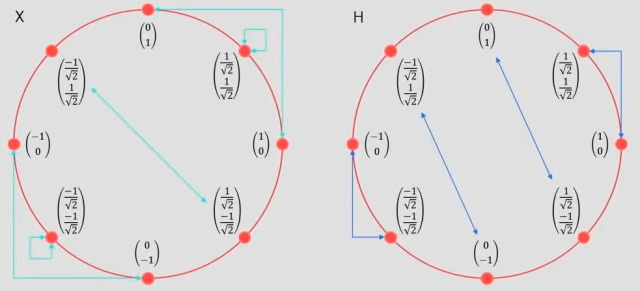
\includegraphics[width=.75\linewidth]{qt-unit-circle.jpg}
    \label{fig:qt-unit-circle}
    \caption{The Map for Moving Q-Bits around}
\end{figure}
\end{frame}

\section{Messing with QC}

\begin{frame}
\frametitle{IBM's API}
\href{https://qiskit.org/}{Qiskit} is bae.

You write QASM (Quantum-ASM) files and Qiskit runs them on a local simulator or online on a real quantum computer.

There is an online interface: \href{https://quantumexperience.ng.bluemix.net/qx/editor}{and it's free for like 5 runs on a Quantum computer.}
\end{frame}

\section{An example: the Deutsch Oracle (time-permitting)}

\begin{frame}
\frametitle{The Deutsch Oracle}

Let $f: \{0, 1\} \to \{0, 1\}$ (so $f$ is a bit operator).
How do we know if it's constant? How can you do it on a standard computer?

\end{frame}

\begin{frame}
\frametitle{The Deutsch Oracle: the Quantum Advantage}

Let $f: \{0, 1\} \to \{0, 1\}$ (so $f$ is a bit operator).
How do we know if it's constant?

One query? He superpose.

\end{frame}

\begin{frame}
\frametitle{The Deutsch Oracle: Reversibility}

$f(x) = 0$ is not reversible.

\begin{block}{Reversibility Hack}
    The hack: operate on two bits: $g(\ket{0, x}) = \ket{f(x), x}$
    The idea is that the 0 bit is the output wire and $x$ the input.
\end{block}

This $g$ is reversible. (Only proof I know: matrices.)

Asking about $g$ is equivalent to asking about $f$, but now you can use quantum operators.

\end{frame}

\begin{frame}
\frametitle{The Deutsch Oracle: What the Constant Functions Look Like}

\begin{block}{Constant 0}
nothing on either wire.
\end{block}

\begin{block}{Constant 1}
$X$ (the flip) on the output wire.
\end{block}

\end{frame}

\begin{frame}
\frametitle{The Deutsch Oracle: What the Variable Functions Look Like}

\begin{block}{Identity}
output = CNOT(input, output)
\end{block}

\begin{block}{Negation}
output = Not(CNOT(input, output))
\end{block}

\end{frame}

\begin{frame}
\frametitle{The Deutsch Oracle: Solution}

\begin{block}{Solution}
input = Hadamard(second bit of g(Hadamard(1), Hadamard(1))

input is 1 iff $g$ constant.
\end{block}

\begin{figure}
    \centering
    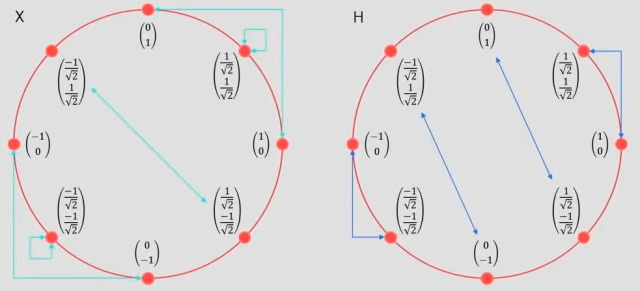
\includegraphics[width=.75\linewidth]{qt-unit-circle.jpg}
    \label{fig:qt-unit-circle}
    \caption{The Map for Moving Q-Bits around}
\end{figure}
\end{frame}

\begin{frame}
\frametitle{The Deutsch Oracle: How the CNOT Works}

\begin{align*}
    C \left(\begin{pmatrix}{1 \over \sqrt{2}} \\{-1 \over \sqrt{2}}\end{pmatrix}
        \otimes \begin{pmatrix}{1 \over \sqrt{2}} \\{-1 \over \sqrt{2}}\end{pmatrix}\right)
    &= C \begin{pmatrix}1/2 \\ -1/2 \\ -1/2 \\ 1/2 \end{pmatrix}
    = {1 \over 2}
        \begin{pmatrix}
        1 & 0 & 0 & 0 \\
        0 & 1 & 0 & 0 \\
        0 & 0 & 0 & 1 \\
        0 & 0 & 1 & 0 \\
        \end{pmatrix}
        \begin{pmatrix}1 \\ -1 \\ -1 \\ 1 \end{pmatrix}\\
    &= {1 \over 2}
        \begin{pmatrix}1 \\ -1 \\ 1 \\ -1 \end{pmatrix}
    = \left(\begin{pmatrix}{1 \over \sqrt{2}} \\{1 \over \sqrt{2}}\end{pmatrix}
        \otimes \begin{pmatrix}{1 \over \sqrt{2}} \\{-1 \over \sqrt{2}}\end{pmatrix}\right)
\end{align*}

\end{frame}

\begin{frame}
\frametitle{The Deutsch Oracle: Why Care?}
It turns out you can do this for functions with $n$ inputs.
Shor's algorithm uses this to factor.
\end{frame}

\begin{frame}
\frametitle{References}
\footnotesize{
\begin{thebibliography}{99} % Beamer does not support BibTeX so references must be inserted manually as below
\bibitem[WIRED, 2018]{5-levels} WIRED (2018)
\newblock Quantum Computing Expert Explains Once Concept in 5 Levels of Difficulty
\newblock \emph{youtube.com} \url{https://www.youtube.com/watch?v=OWJCfOvochA}
\bibitem[Microsoft, 2018]{long-video} Microsoft Research (2018)
\newblock Quantum Computing for Computer Scientists
\newblock \emph{youtube.com} \url{https://youtu.be/F_Riqjdh2oM}
\bibitem[Tatourian, 2018]{img-blog} Alan Tatourian (2018)
\newblock Quantum Computing for Computer Scientists
\newblock \emph{tatourian.blog} \url{https://tatourian.blog/2018/09/01/quantum-computing-for-computer-scientists/}
\bibitem[Cleve]{q-complexity} Richard Cleve
\newblock An Introduction to Quantum Complexity Theory
\newblock \emph{University of Calgary} \url{https://cds.cern.ch/record/392006/files/9906111.pdf}
\bibitem[Quanta, 2018]{q-verification} Erica Klarreich
\newblock Graduate Student Solves Quantum Verification Problem
\newblock \emph{Quanta Magazine} \url{https://www.quantamagazine.org/graduate-student-solves-quantum-verification-problem-20181008/}
\end{thebibliography}
}
\end{frame}

\begin{frame}
\Huge{\centerline{The End}}
\end{frame}

\end{document}
